% !TeX root = ../../../main.tex

The methodology adopted by the \acrlong{nnpdf} has already been described in
its publications, \cite{Forte:2002fg,Ball:2008by}, and in dedicated reviews,
\cite{Forte:2020yip,Ethier:2020way}.
%
Therefore, it would be redundant to add too many details here, that can be
easily found in references, but it is relevant to summarize the main points,
for the subsequent discussion.

The primary challenge in switching from polynomial parametrization\footnote{
  Or parametrization over a fixed basis of functions, more in general.
} to \nn consists in the uncertainty propagation.
Indeed, the first step would be to establish a training algorithm, but, while
the fixed parametrizations require an explicit choice, the \nn comes with its
own efficient training algorithm.
%
It is in no way unique, and there are many options available, but there is no
need for a dedicated development.
The exact algorithm selection becomes part of the methodology, and it is once
more a source of arbitrariness, but there are suitable strategies to educate
this choice, and sometimes it is also driven by consistent technical
considerations.

Before explaining the uncertainty propagation technique it is worth noticing
that the most renowned and usual applications of \acrshortpl{nn} aim to
determine an unknown function, but the details of the learnt function are not
particularly relevant, while it is relevant to evaluate it on a specific subset
of inputs, settling the \textit{task} to be performed by the trained network.
%
In the case of the \pdfs, all values of the functions are relevant, since a
large enough set of physical observables is potentially sensible to all its
analytical features.
%
Moreover, being able to manually examining the function can help in inferring
specific properties of the hadrons.
%
So, the final step of an \nn fit is to evaluate the function on a sufficiently
complete set of inputs, originating a function set by means of interpolation.

In this context, fixed parametrization fits are no different, because after
determining the parameters in a Hessian fit, they also evaluate the resulting
functions.
%
To propagate the uncertainty, an Hessian fit require to determine the main
eigenvectors for the minimized quantity, generating a Gaussian distribution
that approximate the uncertainty on the fitted parameters in a neighborhood of
the best fit.

For an \nn fit this is not technically available, because of the large number
of parameters involved. And even when it would be possible, it is not
recommended to follow the classical approach, since many parameters might be
poorly constrained, but with a negligible impact on the value of the \pdfs.
%
Therefore, \nnpdf proposed a more direct approach: since the distribution in
the value of the \pdf is derived from the data distribution, it is possible to
start from an alternative representation of this distribution.
%
As illustrated in \cref{fig:gp/nnpdf}, the data are then fluctuated, according
to their distribution, and many samples of the whole dataset are taken, each
one containing one and only one value for each experimental data point (i.e.\
each sample is a single extraction from the joint distribution of all
experimental data).
%
This samples are called \textbf{\textit{data replicas}}.
%
After that, one \nn is fitted to each replicate, and the resulting set of
trained \acrshortpl{nn}, called \textbf{\textit{\nn replicas}} are gathered,
and they are the determined \mc representation of the \pdfs distribution.
%
In particular, this procedure associates to each point in the \pdfs domain a
set of values (the \nn replicas), that should be interpreted as a sample of the
\pdfs distribution for that point.

\begin{figure}
	\centering
	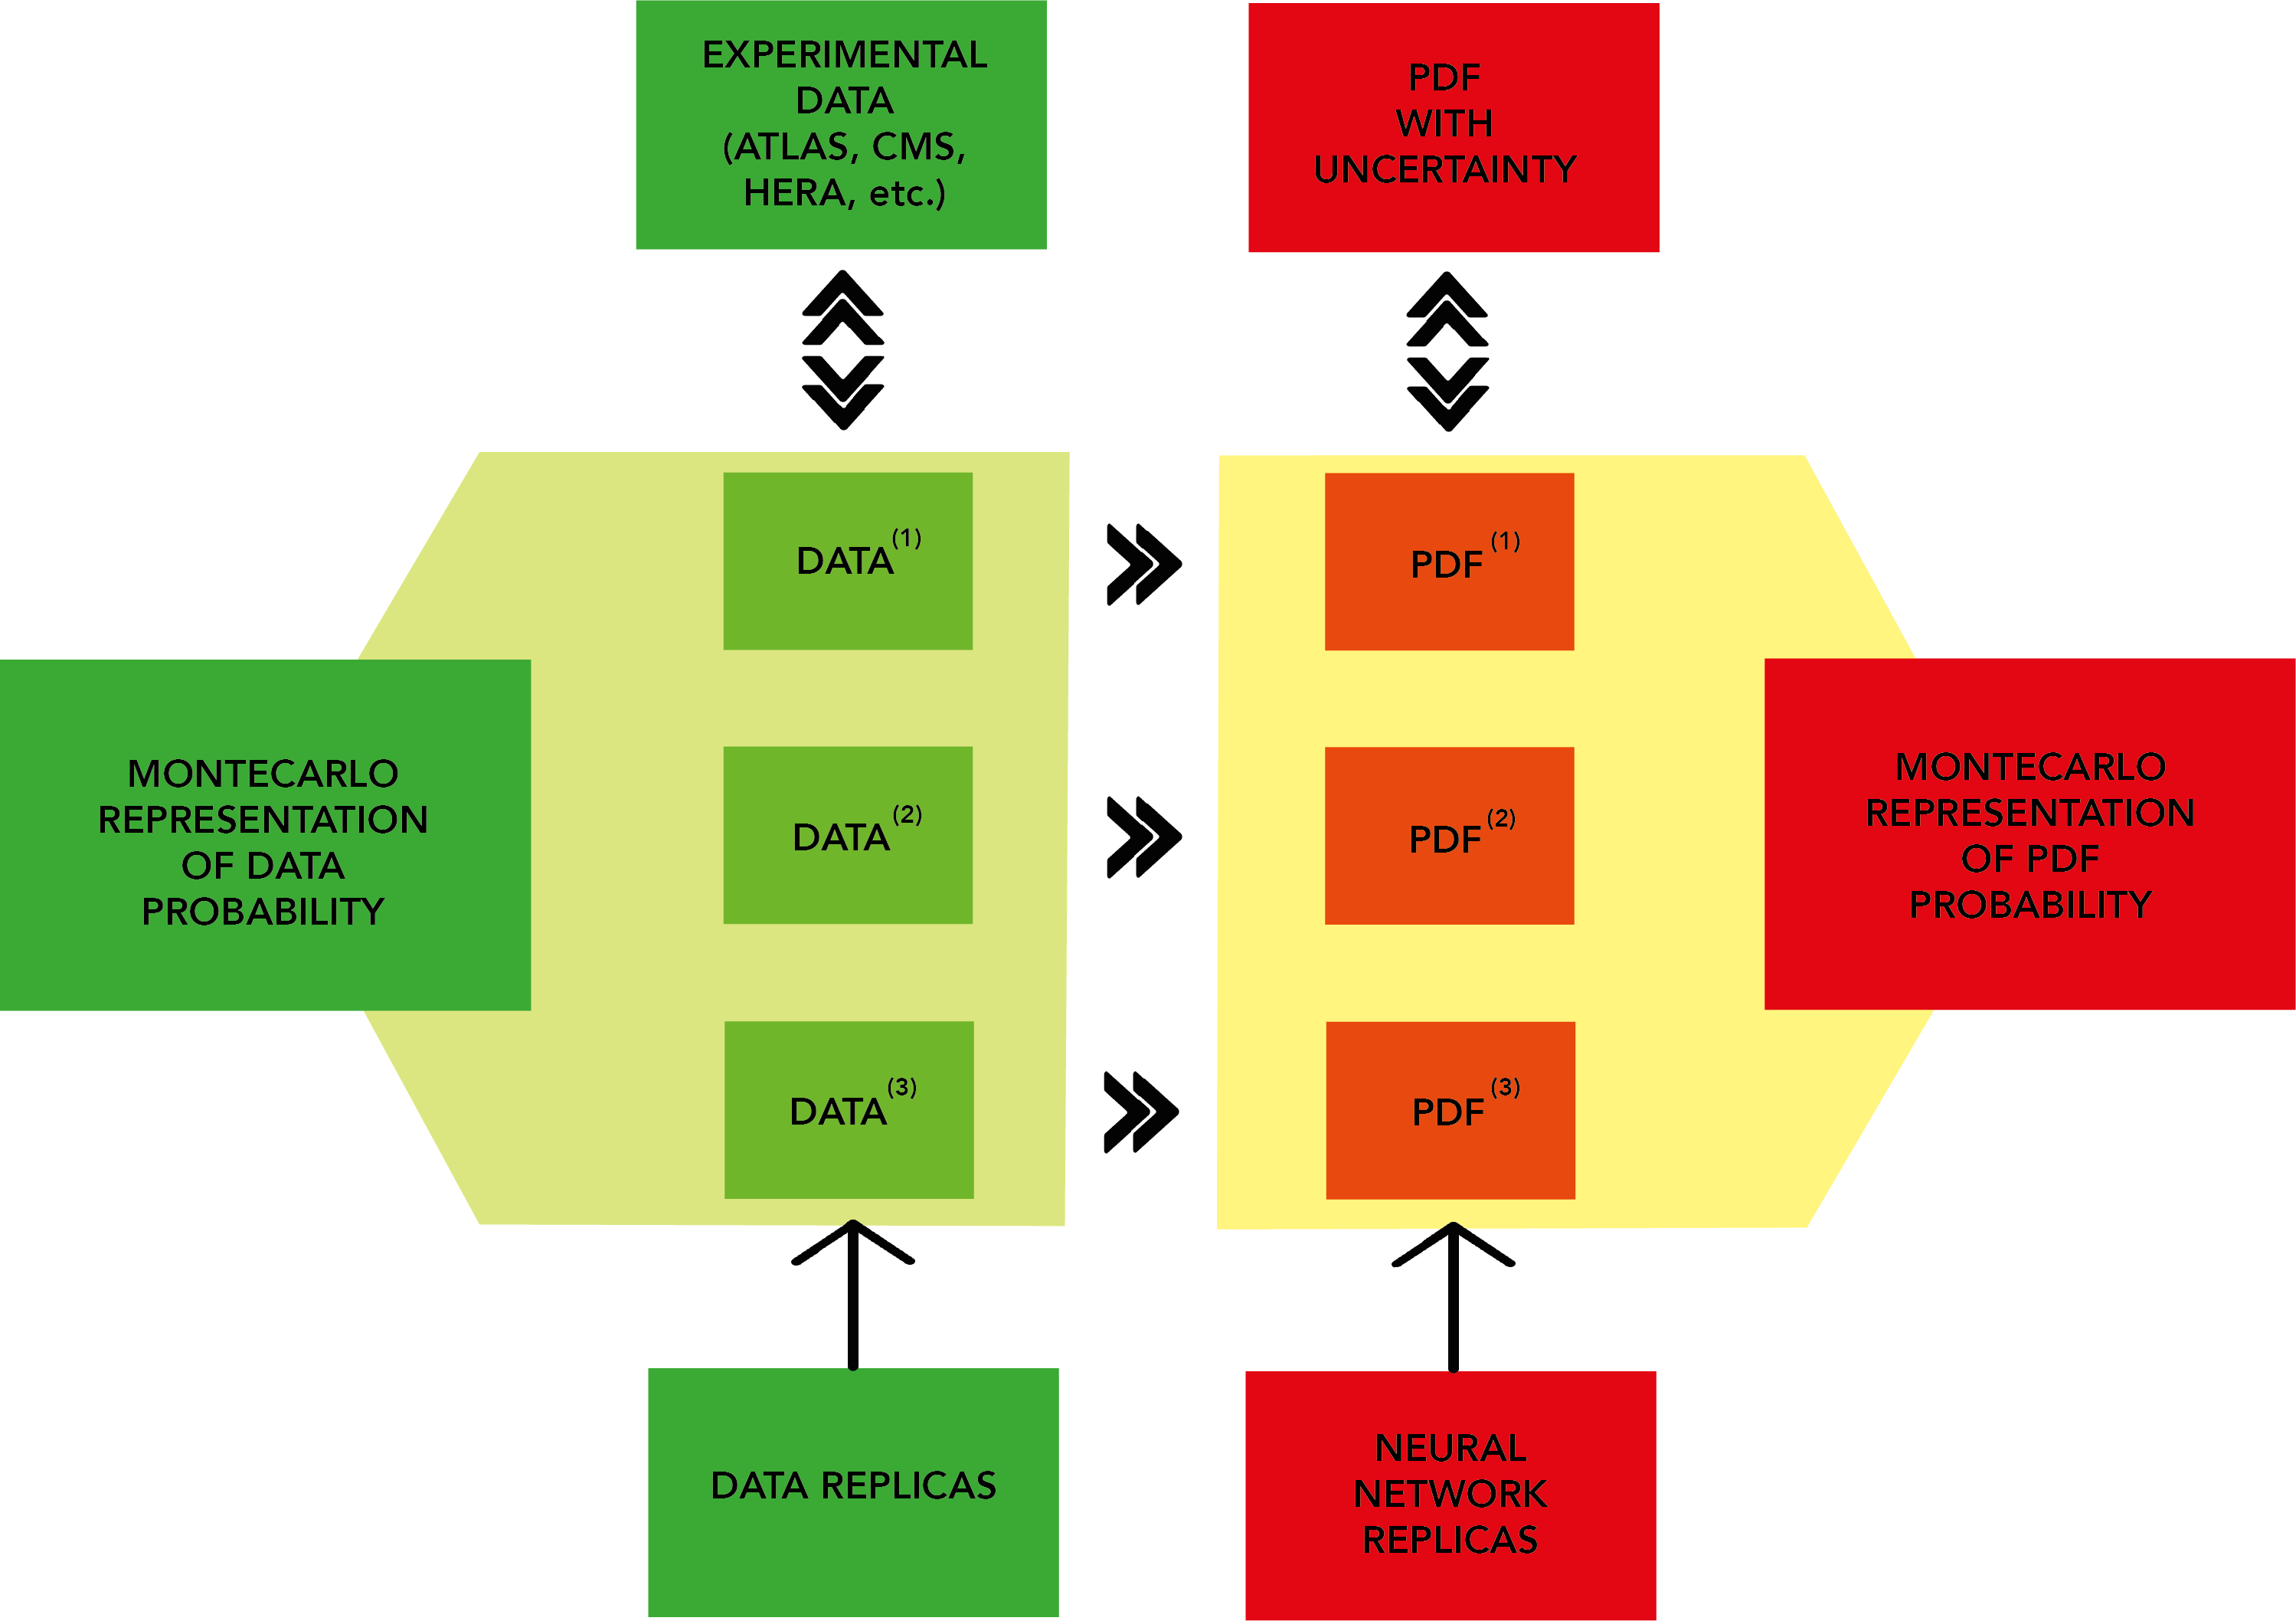
\includegraphics[width=\hsize]{ch-gp/nnpdf-strategy}
	\caption{
    \nnpdf uncertainty propagation methodology, one of the most important key
    points of \nnpdf methodology.
    Picture available on the collaboration website
    \url{http://nnpdf.mi.infn.it/research/general-strategy/}.
	}
	\label{fig:gp/nnpdf}
\end{figure}

As thoroughly discussed in \cite{DelDebbio:2021whr}, this boils down to solve
the \textit{inverse problem} for the \pdfs: the map from \pdf space to data
space is known, and it consists in the theory prediction. So the fit is
essentially inverting this map, constrained with some assumptions.
%
Applying the inverse\footnote{
  The inverse map is not a unique one, since the \nn may obtain different
  minima according to its initialization.
  If this is done randomly, the distribution of the initialization assigns a
  certain probability to each possible minimum, creating a probabilistic
  inverse, that will convolute the data distribution in the result.
  This becomes clearer in the Bayesian framework in \cref{sec:gp/bayes}, where
  this further probability can be essentially identified with the prior. 
} to each data replica the distribution is propagated from one space to the
other.

\paragraph{Closure tests} However, the training algorithm for the \nn is
sufficiently sophisticated to introduce a further level of indirectness, that
makes harder to understand which features of the input dataset is causing a
specific behavior in the output distribution.
%
Because of this partial loss of explainability (part of it is already in the
size of the dataset, and the lack of a one-to-one mapping caused by
convolutions), the methodology requires to be validated in a more systematic
way.
%
\nnpdf is doing this employing \textit{closure tests}, explained in details in
\cite{DelDebbio:2021whr}.
%
Basically, a set of fake data is generated by a fake underlying \textit{truth},
chosen to be a reasonable \pdf set (usually a set by a different collaboration)
applying the same theory predictions used in the fit, and the final result is
compared to the starting point.

This exercise is possible at many levels: 
\begin{description}
  \item[level 0] using directly the mock truth, or
  \item[level 1] fluctuating it, to emulate how the experimental uncertainty is
    affecting the estimate of central values, or
  \item[level 2] fluctuating once more, to obtain the same data replicas used
    in a regular fit
\end{description}

Closure tests have a great power in assessing the faithfulness of the
uncertainties established by a given methodology.
%
It is important to remark that what is tested is not if there would exist an
alternative methodology that could led to smaller uncertainties, but only if
the chosen one produces an estimate of the uncertainty that is compatible with
the expected shift of the central value from the underlying truth.
%
Then, two very different methodologies, one obtaining much bigger errors than
the other from the same dataset, can both pass the closure test, if their error
is consistent with the actual shift from the truth: big uncertainty associated
to a big shift, and conversely.

Nevertheless, also closure tests have some limitations, since they test the
methodology with the assumption of perfectly consistent data, and accepting
the perturbative theory predictions, truncated at a fixed order, as a prompt
for the full theory, generating fake data for that \pdf.
%
These two elements introduce an ambiguity in the outcome of the closure tests
themselves, that is possible to alleviate studying how it behaves when specific
inconsistencies are injected (this is actually a work currently in progress,
being performed by \nnpdf members).

\subsection{Generalization}

As in other classical machine learning problems, also for \pdfs there is a
fundamental concern, that goes beyond the loss function minimization: how much
does the predictions extend, beyond the region strictly covered by data?

The first instance of this issue is interpolation itself, since an extremely
aggressive optimization can generate an incredibly noisy result, matching
anyhow all the points in the dataset.
%
This is partially prevented by the structure of the network itself, and its
training algorithm: in the case of \nnpdf there is no explicit penalty term
imposing smoothness in the loss function.
%
The rest is done by the \textit{training-validation} split. As it is customary
for many machine learning applications, data are split in the two sets, and
only one of the two is passed to the optimizer, while the other is observed
during the training, in order to interrupt the process before learning the
noise, and prevent \textit{over-fitting}.
%
Despite being very common, there is not a full analytical understanding for
this method, or for the \nn training more in general, and many
counter-intuitive are still being investigated (e.g.\ double descent, or
multiple in general).
So, the final and most reliable proof of good interpolation properties comes
from the closure tests.

A second instance lies in the extrapolation region. 
%
Since this region is not directly controlled by data, or at least very little,
it is largely undetermined, but it is important for \pdfs uncertainties to be
reliable also in this region, usually heavily affecting \bsm searches.
%
Being reliable means to be large enough to cover unobserved features of the
\pdfs, without completely forgetting the few constraints coming from the sum
rules.
%
To check the fidelity of these portions of the final product, a different kind
of tests is employed: the dataset is chronologically segmented, and they are
incrementally included in the input of the \nn, finally comparing the various
results.
%
This type of checks have been called \textit{future tests}, and the essential
idea consist to check how faithful are the extrapolation uncertainties, since
the extrapolation region of a chronologically prior fit will intersect the data
region of a later one.
%
In practice, despite \nnpdfr{4.0} being significantly smaller than those in the
other \pdf set, this is mostly limited to the data region, and the increased
flexibility prevents an extreme extrapolation, decoupling the two regions, as
much as it is allowed by sum rules.
This is shown and exemplified quite well in the Drell--Yan forward-backward
asymmetry study, presented in \cref{ch:afb}.

It is worth to remark once more that there are many possible variations, whose
results can span wide space of solutions.
In order to avoid arbitrary choices, inspired by subjective opinions or
\textit{human experience} (potentially reliable, but certainly hard to quantify
and systematically improve), in \nnpdfr{4.0} a large enough space of
hyperparameters has been considered, and they have been hyperoptimized (also
standard practice, though computationally expensive) based on a grid search.
%
This also contribute to improve the generalization power of the full procedure,
since also the methodology parameters have been systematically optimized for
this task.

\subsection{Minor improvements}

- sampling with negative values
- fast thcovmat construction
